\documentclass[fleqn,xcolor={usenames,dvipsnames},notes,aspectratio=169]{beamer} % [notes=only]
\usepackage{amsmath} % {amssymb,amsfonts}
\usepackage{eurosym}

% \usepackage{array,adjustbox} % url

% \usepackage{pifont,marvosym} % \ding

% \usepackage{multimedia}
% \usepackage[normalem]{ulem}
% \usepackage{framed,color,ragged2e}
% \usepackage[absolute,overlay]{textpos}
% \definecolor{shadecolor}{rgb}{0.8,0.8,0.8}

\usetheme{boxes}
\setbeamertemplate{navigation symbols}{}
% \useinnertheme{circles}

\usepackage{xcolor}
\usepackage{tikz}
\usetikzlibrary{shapes,arrows}
\usetikzlibrary{tikzmark,positioning}
\usetikzlibrary{calc}

\newtheorem*{rawnamedtheorem}{\therawnamedtheorem}
\newcommand{\therawnamedtheorem}{\error}
\newenvironment{namedtheorem}[1]{\renewcommand{\therawnamedtheorem}{#1}
   \begin{rawnamedtheorem}}
  {\end{rawnamedtheorem}}


\title{Applying verifiable random functions}
% \subtitle{Cryptography for killing proof-of-work}
% \subtitle{Technologies to secure the future Internet}


\author[Burdges]{Jeff Burdges}
\institute{
  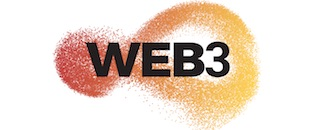
\includegraphics[scale=0.25]{../logos/web3logo.jpg}. % web 3 foundation
}
\date{30.12.2019} % 12:00 in OIO Stage

% \newcolumntype{R}[2]{%
%     >{\adjustbox{angle=#1,lap=\width-(#2)}\bgroup}%
%     l%
%     <{\egroup}%
% }
% \newcommand*\rot{\multicolumn{1}{R{45}{1em}}}% no optional argument here, please!

\def\signed #1 (#2){{\leavevmode\unskip\nobreak\hfil\penalty50\hskip2em
  \hbox{}\nobreak\hfil\normalfont --#1 (#2)%
  \parfillskip=0pt \finalhyphendemerits=0 \endgraf}}
% https://tex.stackexchange.com/questions/13756/quote-environment-with-reference-at-the-end-right



\newcommand{\algo}[1]{\ensuremath{\mathsf{#1}}}
\newcommand{\VRF}{\algo{VRF}} 
\newcommand{\RingVRF}{\algo{RingVRF}} 
\newcommand{\Sign}{\algo{Sign}} 
\newcommand{\Verify}{\algo{Verify}} 
\newcommand{\KeyGen}{\algo{KeyGen}} 
\newcommand{\sk}{\ensuremath{\mathsf{sk}}}
\newcommand{\pk}{\ensuremath{\mathsf{pk}}}


\begin{document}


{\setbeamertemplate{footline}{}
\begin{frame}
\titlepage
\end{frame}
}
\setcounter{framenumber}{0}


% Implementation: GNU Taler \\
% \qquad \url{http://taler.net} \qquad \url{http://demo.taler.net}


\begin{frame}

We authenticate messages using either
\begin{itemize}
\item signatures like GPG/PGP, or else
\item message authentication codes (MACs), like anything sensible.
\end{itemize}

\bigskip 

MACs are (deterministic) functions, while signatures
\begin{itemize}
\item provide non-repudiation, and 
\item admit verification from only public key, not a shared secret key,
\end{itemize}

\end{frame}


\begin{frame} %{}

A MAC combines a shared secret key with ciphertext to produce a {\em tag} $f_k(m)$, \\
which must ``resist existential forgery under chosen-plaintext attack,'' \\
\hspace*{3pt} and not leak anything about the key in particular.

\bigskip

Some but not all MACs are pseudo-random function families (PRF), meaning 
no known algorithm has non-negligible odds to distinguish between $f_k$ and a ``random oracle''.

\end{frame}


\begin{frame}

A {\em verifiable random function} (VRF) is a pseudo-random function family but \\
parameterized by public-secret key pairs.  
\begin{itemize}
\item $(\pk,\sk) \leftarrow \VRF.\KeyGen$
\item $(\omega,\pi) \leftarrow \VRF.\Sign_{\sk}(\alpha)$
\item $\VRF.\Verify_{\pk}(\omega,\pi)$
\end{itemize}

\medskip

In other words, VRFs are public-key analogs of a strong keyed hash functions: % \\ such as some MACs, meaning
\begin{itemize}
\item anyone with the public key can verify the correctness, but
\item only the secret key holder could compute the output $\omega$.
\end{itemize}

\pause\bigskip

$$ m \mapsto \sk \ H_1(m) $$

% $e(s,G_2) = e(H_1(m),A)$

\end{frame}


\begin{frame}{VRF: DLEQ Proof}
  
  \begin{columns}
    % \small
   \begin{column}{0.5\textwidth}
    {\em (1) Key generation} \\
    \begin{itemize}
    \item[$\circ$] Secret key $a \in \mathbb{Z} \mod q$
    \item[$\circ$] Public key $A = a B$ 
    \end{itemize}
    \bigskip
    {\em (2) Signing} \\
    \begin{enumerate}
    \item Set $M := H_1(m)$ and $\omega := a M$
    \item Choose random nonce $k$
    \item Set $c := H_0(M, A, \omega, k B, k M)$
    \item Set $s := k - c a$
    \item Signature $(\omega,c,s)$
    \end{enumerate}
  \end{column}
   \begin{column}{0.5\textwidth}
    {\em (2) Verification} \\
    \begin{enumerate}
    \item $M := H_1(m)$ 
    \item $U := c A + s B$
    \item $V := c \omega + s M$
    \item $c := H_0(M, A, \omega, U, V)$
    \end{enumerate}
   \end{column}
  \end{columns}
  \bigskip
  {\it Making NSEC5 Practical for DNSSEC} by ...
  Schnorrkel:  https://github.com/w3f/schnorrkel/blob/master/src/vrf.rs
 
 \end{frame}


\def\rh{\textcolor{red}{h}}
\def\yh{}

\begin{frame}{Aside: Cofactors doh! }

  \begin{columns}
   % \small
   \begin{column}{0.5\textwidth}
    % {\em (1) Key generation} \\
    % \begin{itemize}
    % \item[$\circ$] Secret key $a \in \mathbb{Z} \mod q$
    % \item[$\circ$] Public key $A = a B$ 
    % \end{itemize}
    % \bigskip
    {\em (2) Signing} \\
    \begin{enumerate}
    \item Set $M := \rh H_1(m)$ and $\omega := a M$
    \item Choose random nonce $k$
    \item Set $c := H_0(M, \yh A, \omega, \yh k B, k M)$
    \item Set $s := k - c a$
    \item Signature $(\omega',c,s)$ where $\omega' := \rh^{-1} \omega$
    \item Output $H_0(M, A, \omega)$
    \end{enumerate}
   \end{column}
   \begin{column}{0.5\textwidth}
    {\em (2) Verification} \\
    \begin{enumerate}
    \item $\omega := \rh \omega'$ 
    \item $M := \rh H_1(m)$ 
    \item $U := c A + s B$
    \item $V := c \omega + s M$
    \item $c := H_0(M, \yh A, \omega, \yh U, V)$
    \item Output $H_0(M, A, \omega)$
    \end{enumerate}
   \end{column}
  \end{columns}
  \bigskip
  Or else check $\textcolor{red}{q} \omega = 0$ but that's slow.
  \smallskip
  Who does not do this?
  \begin{enumerate}
  \item {V(X)Ed25519} by Trevor Perrin
  \item https://tools.ietf.org/html/draft-irtf-cfrg-vrf-04 \\
        by S. Goldberg, Reyzin, Papadopoulos, Vcelak
  \end{enumerate}

\end{frame}


\begin{frame}{VRFs yield and need randomness beacons}
\begin{center} 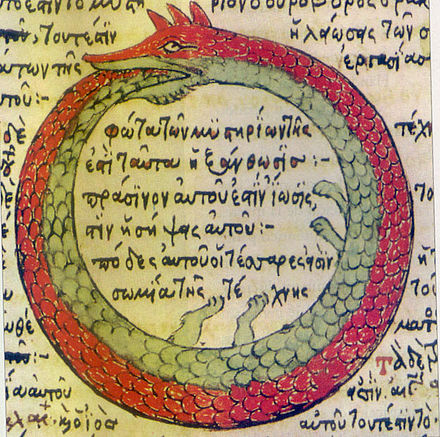
\includegraphics{../pics/ouroborous/440px-Serpiente_alquimica.jpg} \end{center}
\end{frame}


\begin{frame} % {Proof-of-stake Randomness beacon $r_e$}

  \begin{columns}
   \begin{column}{0.35\textwidth}
   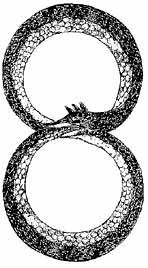
\includegraphics[width=0.9\textwidth]{../pics/ouroborous/ouroboros_double.jpg}
   \end{column}
   \begin{column}{0.65\textwidth}
    {\em By epoch $e-1$,} \\ \hspace*{3pt} 
     any participants for epoch $e+2$ \\ \hspace*{3pt} 
     must declare their VRF public key $\pk$.

    \bigskip\bigskip
    
    {\em At time $t$ in epoch $e$,} \\ \hspace*{3pt}
     $\pk$ makes block with $(\omega_t,\pi_t) = \VRF.\Sign_{\sk}(r_e || t)$ \\ \hspace*{3pt}
     {\em if} $H_0(M, A, \omega_t) < c$. % where $c$ set by their stake.

    \bigskip\bigskip
    {\em In epoch $e+1$,} \\ \hspace*{3pt}
     we set $r_{e+2} = H(\omega_t)$
    
   \end{column}
  \end{columns}

\end{frame}


\begin{frame}

We made a ranodmness beacon and a blockchain ..

\medskip 

\hspace*{3pt} .. but can we do anything useful?

\pause\bigskip\bigskip

Tor has a bandwidth authority run of by 9ish people

\end{frame}


% \begin{frame}{What is a mix network?}
% \begin{enumerate}
% \item Message oriented
% \item Unreliable packet switching network 
% \item Layered encryption in a single packet
% \item Added latency per hop, aka they mix
% \end{enumerate}
% \end{frame}


\begin{frame}{Mix networks}
\begin{center}
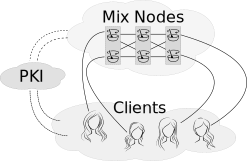
\includegraphics[width=0.85\textwidth]{../pics/mix/initial}
\end{center}
\end{frame}


\begin{frame}{Loopix Achitecture}
\begin{center}
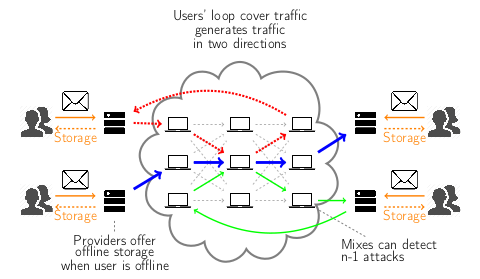
\includegraphics[trim=0 0 0 50,clip,width=\textwidth]{../pics/loopix/achitecture}
\end{center}

%\medskip
\hspace*{3pt} Ania Piotrowska, Jamie Hayes, Tariq Elahi, Sebastian Meiser, and
\hspace*{3pt} George Danezis. {\em The Loopix Anonymity System} Usenix 26, 2017.

\end{frame}


\begin{frame}

We have a global PKI in which some, but not all, mix nodes
 register a key $A = a B$.
% \\ \hspace*{3pt} register a VRF public key $A = a B$.

\smallskip

As above, they run a random bacon with output $r_e$ in epoch $e$.

\pause\bigskip\medskip

Run our VRFR lots: \\ \hspace*{3pt} 
For $i < 2^{10\mathrm{ish}}$, $A$ computes \\ \hspace*{3pt} 
 VRF inputs $M_i = H_1(r_e || \mathrm{"LC"} || i)$, and \\ \hspace*{3pt} 
 VRF outputs $\omega_i = a M$, so..\\ 

\bigskip

Send cover packets seeded by the results: \\ \hspace*{3pt} 
Set $s_i) := H_0(M_i, A, \omega_i)$. 
If $s_i< c$ then $A$ makes \\ \hspace*{3pt} 
 a loop cover packet $p_i$ using the CSPRNG $\mathsf{ChaCha20}(s_i)$, \\ \hspace*{3pt} 
 which $A$ sends whenever the cover traffic scheme dictates.

\bigskip

Our PKI and CSPRNG determine $p$ completely.

\end{frame}


\begin{frame}

All mixnets need replay protection, so 

\bigskip

Announce winning packets in some future epoch $e+5$: \\ \hspace*{3pt} 
If $H(s_i || r_{e+5}) < c'$ for some $i$ then \\ \hspace*{3pt} 
 $A$ publishes VRF outputs $\omega_i$ with proofs $\pi_i$.

\end{frame}


\begin{frame}

\end{frame}



\end{document}






\begin{frame}{BLS signatures}
  \begin{columns}
    \small
   \begin{column}{0.5\textwidth}
    {\em (0) Paramaters} \\
    \begin{itemize}
    \item[$\circ$] Elliptic curve $E$ over a field of \\
          characteristic $p$.
    \item[$\circ$] $G_1 < E_p$ and $G_2 < E_{p^2}$ order $q$ prime.
    \item[$\circ$] $B_1 \in G_1$ and $B_2 \in G_2$
    \item[$\circ$] $e : G_1 \times G_2 \to \mathbb{F}_{p^{12}}$ \\
          $e(X+Y, Z) = e(X,Z) e(Y,Z)$ \\
          $e(X, Y+Z) = e(X,Y) e(X,Z)$ \\
          $e(a X, b Z) = e(X,Z)^{a b}$
    \item[$\circ$] Hash-to-curve $H_1 : * \to G_2$
    \end{itemize}
  \end{column}
  \begin{column}{0.5\textwidth}
    {\em (1) Key generation} \\
    \begin{itemize}
    \item[$\circ$] Secret key $a \in \mathbb{Z} \mod q$
    \item[$\circ$] Public key $A = a B_2$ 
    \end{itemize}
    {\em (2) Sign} \\
    \begin{enumerate}
    \item[$\circ$] Signature $s' := a H_1(m)$.
    \end{enumerate}
    {\em (3) Verification} \\
    \begin{enumerate}
    \item[$\circ$] $e(s,G_2) = e(H_1(m),A)$? \\ \smallskip
    \qquad $e(H_1(m),G_2)^a$
    \end{enumerate}
   \end{column}
  \end{columns}
\end{frame}


\begin{frame}{BLS blind signatures}
  \begin{columns}
    \small
   \begin{column}{0.5\textwidth}
    {\em (1) BLS key generation} \\
    \begin{itemize}
    \item[$\circ$] Secret key $a \in \mathbb{Z} \mod q$
    \item[$\circ$] Public key $A = a B_2$ 
    \end{itemize}
    \bigskip
    {\em (3) Blind signing} \\
    \begin{enumerate}
    \item Receive $m'$.
    \item Send signature $s' := a m'$.
    \end{enumerate}
  \end{column}
   \begin{column}{0.5\textwidth}
    {\em (2) Blinding} \\
    \begin{enumerate}
    \item Create $a \in \mathbb{Z} \mod q$
    \item Send $m' := b H_1(m)$.
    \end{enumerate}
    {\em (4) Unblinding} \\
    \begin{enumerate}
    \item Receive $s'$.
    \item Compute $s := (b^{-1} \mod q) s'$.
    \end{enumerate}
    {\em (5) Verification} \\
    \begin{enumerate}
    \item[$\circ$] $e(s,G_2) = e(H_1(m),A)$.
    \end{enumerate}
   \end{column}
  \end{columns}
\end{frame}



